%%%%%%%%%%%%%%%%%%%%%%%%%%%%%%%%%%%%%%%%%%%%%%%%%%%%%%%%%%%%%%%%%%%%%%%%%%%%%%%%%%%%%
% Reinforcement Learning
%
% Introduction to MDPs, finite MDPs, infinite MDPs
% Semi MDPs
% Partially Observable MDPs
%
%%%%%%%%%%%%%%%%%%%%%%%%%%%%%%%%%%%%%%%%%%%%%%%%%%%%%%%%%%%%%%%%%%%%%%%%%%%%%%%%%%%

\section{The Reinforcement Learning Problem}

In general terms, reinforcement learning in an industrial setting is simply an agent undergoing meaningful interactions with the process to learn an optimal operating policy.  For added intuition, Figure \ref{fig: simple_rl} shows the information flow of an agent in process control. First, the agent observes some states, $x_t \in \mathcal{X}$, from the environment (some states may be unobservable).  Given $x_t$, the agent performs some controls actions, $u_t \in \mathcal{U}$ and receives a scalar reward signal, $r_{t+1} \in \mathcal{R}$.  Finally, the process will transition to some new states, $x_{t+1}$, given probability $P(x_{t+1}, r_{t+1} | x, u)$.

\begin{figure}[H]
    \centering
    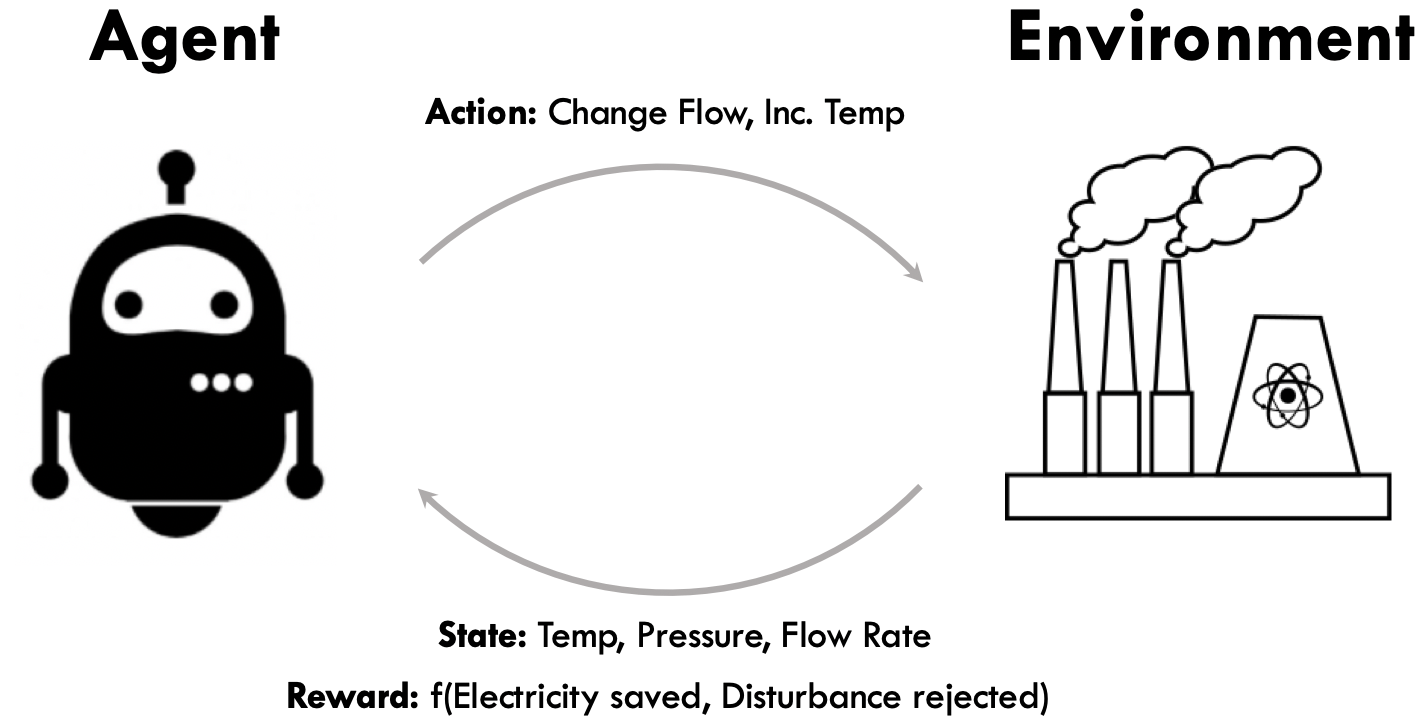
\includegraphics[scale=0.5]{images/ch1/RL.png}
    \caption{Basic setup of reinforcement learning where an agent interacts with the system.}
    \label{fig: simple_rl}
\end{figure}

The three main branches of reinforcement learning solutions are shown in Figure \ref{fig:RL_methods}. Starting from the left, dynamic programming (DP) methods can identify the exact value functions, but require a \textit{perfect system model} and is extremely computationally expensive, even for trivial tasks.  Comparatively, both Monte Carlo (MC) and temporal difference (TD) methods are approximate DP methods.  As such, they are less computationally demanding.  Additionally, MC and TD methods do not assume the presence of a system model and identifies the value functions through interactions with the environment. MC methods find the value functions through averaging the returns generated over many sampled trajectories of states, actions, and rewards.  One drawback is the significant variance in the sampled trajectories. Consequently, this may lead to poor reproducability in highly noisy systems. TD methods combine the best characteristics of DP and MC methods into one unifying approach. Like MC methods, TD learn from sampled data.  Like DP methods, TD performs update steps after each step. However, TD methods typically exhibit large bias (especially during initial learning episodes) due to estimating values through previously estimated values (known as bootstrapping). The general details of each method will be shown throughout this section.  For a comprehensive introduction to each algorithm, see \cite{sutton}.

\begin{figure}[H]
    \centering
    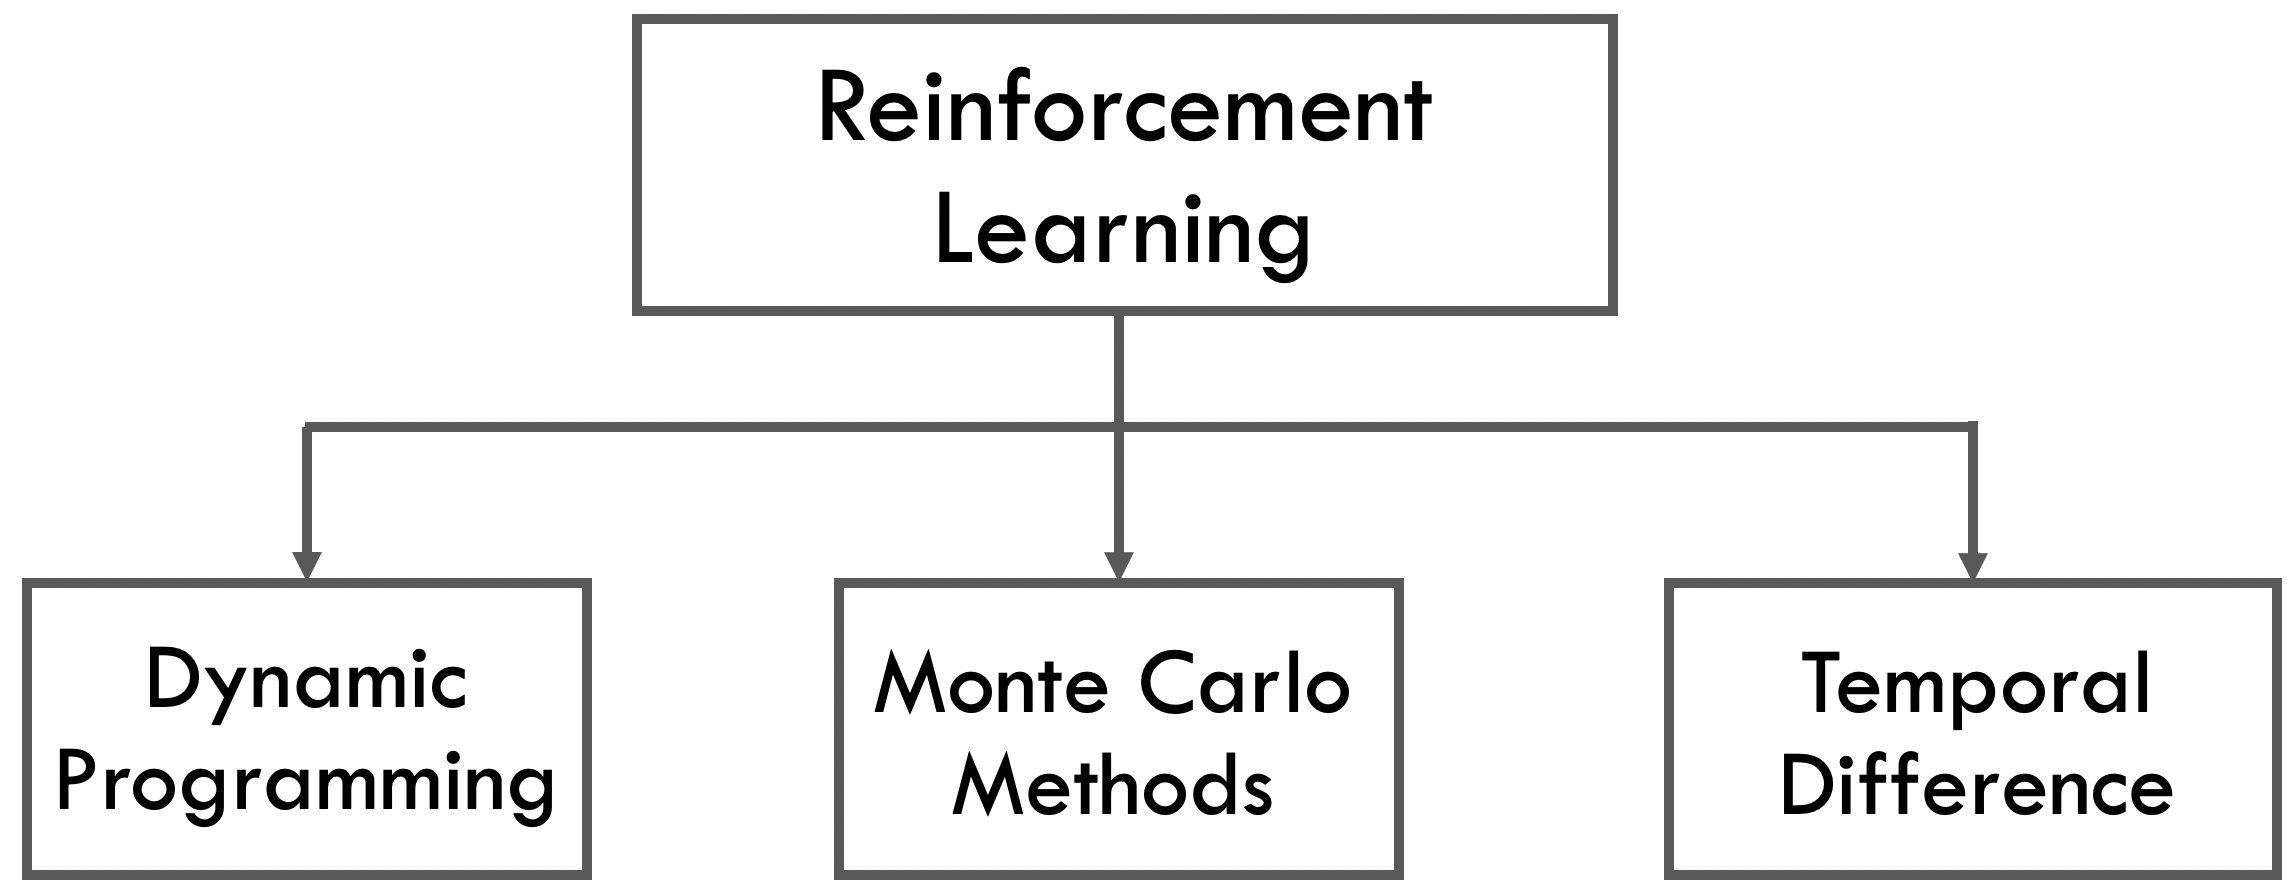
\includegraphics[width=0.6\textwidth]{images/ch1/RL_methods.jpeg}
    \caption{The sub-components of machine learning.}
    \label{fig:RL_methods}
\end{figure}   


\subsection{Dynamic Programming Methods}
Dynamic programming algorithms identify the exact value functions through an iterative procedure using the system dynamics function. In real life applications, DP algorithms are rarely used due to their unreasonable computational cost for even trivial problems. Nevertheless, the ideas of DP serve as the fundamentals for modern approaches. Policy iteration and value iteration are two common techniques in DP.  

As an overview, policy iteration searches for the optimal policy by iterating through infinitely many policies, $\pi \in \Pi$, storing only the policy corresponding to the highest cumulative returns.  The optimal policy is assumed to be found when $G_{\pi}$ can no longer be improved.  Policy iteration is comprised of two phases: policy evaluation and policy improvement. \textbf{Policy evaluation} computes the value functions and cumulative returns of the system under $\pi$ through an iterative approach. Value functions are initialized as 0, and are solved iteratively using:
\begin{equation}
    v_{k+1, \pi}(x) = \mathbb{E}_{\pi}[R_{t+1} + \gamma v_{k, \pi} (x_{k+1})]
\end{equation}
$$ v_0(x) = 0, \; \forall x \in \mathcal{X}$$
where $k$ denotes the $k^{th}$ update.  Here, $v_{k+1, \pi}(x)$ is the predicted value function for $x$ under policy $\pi$ after $k+1$ update steps.  As $k \rightarrow \infty$, $v_{k}(x) \rightarrow v_{\pi}(x)$ for all $x \in \mathcal{X}$ (i.e., the value functions converge to the true value functions under $\pi$). However, there often exists a $\pi'$ where $v_{\pi'}(x) \geq v_{\pi}$.  \textbf{Policy improvement} identifies such situations.  Once identified, current policy $\pi$ will violate the principle of optimality, hence deeming it ineligible for being the optimal policy. Then, the value functions of $\pi'$ will be identified in the next policy evaluation. This procedure will continue iteratively and infinitely until a policy where $v_{\pi^*}(x) \geq v_{\pi \neq \pi^*}(x)$ for all $x \in \mathcal{X}$ is found. After such a policy is identified, it is regarded as the optimal policy.

Figure \ref{fig:policy_iteration} shows a visualization of the policy iteration algorithm.  It can also be described using the following \cite{sutton}:
\begin{equation}
    \pi_0 \xrightarrow{\text{E}} 
    v_{\pi_0} \xrightarrow{\text{I}} 
    \pi_1 \xrightarrow{\text{E}}
    v_{\pi_1} \xrightarrow{\text{I}} 
    \pi_2 \xrightarrow{\text{E}} ... \xrightarrow{\text{I}} 
    \pi^* \xrightarrow{\text{E}}  v^*
\end{equation}
where $\xrightarrow{\text{E}}$ and $\xrightarrow{\text{I}}$ denotes the policy evaluation and policy improvement steps, respectively. From Figure \ref{fig:policy_iteration}, the agent starts with some arbitrary policy and performs policy evaluation. Initially, a large gap exists between $V_{\pi}$ and $\pi$.  As the iterative procedure proceeds, the gap is continuously reduced until $V_{\pi}, \pi \rightarrow V^*(x), \pi^*$. In industrial applications, the required iterative procedure for each policy evaluation is far too expensive for any non-trivial tasks.

\begin{figure}[H]
    \centering
    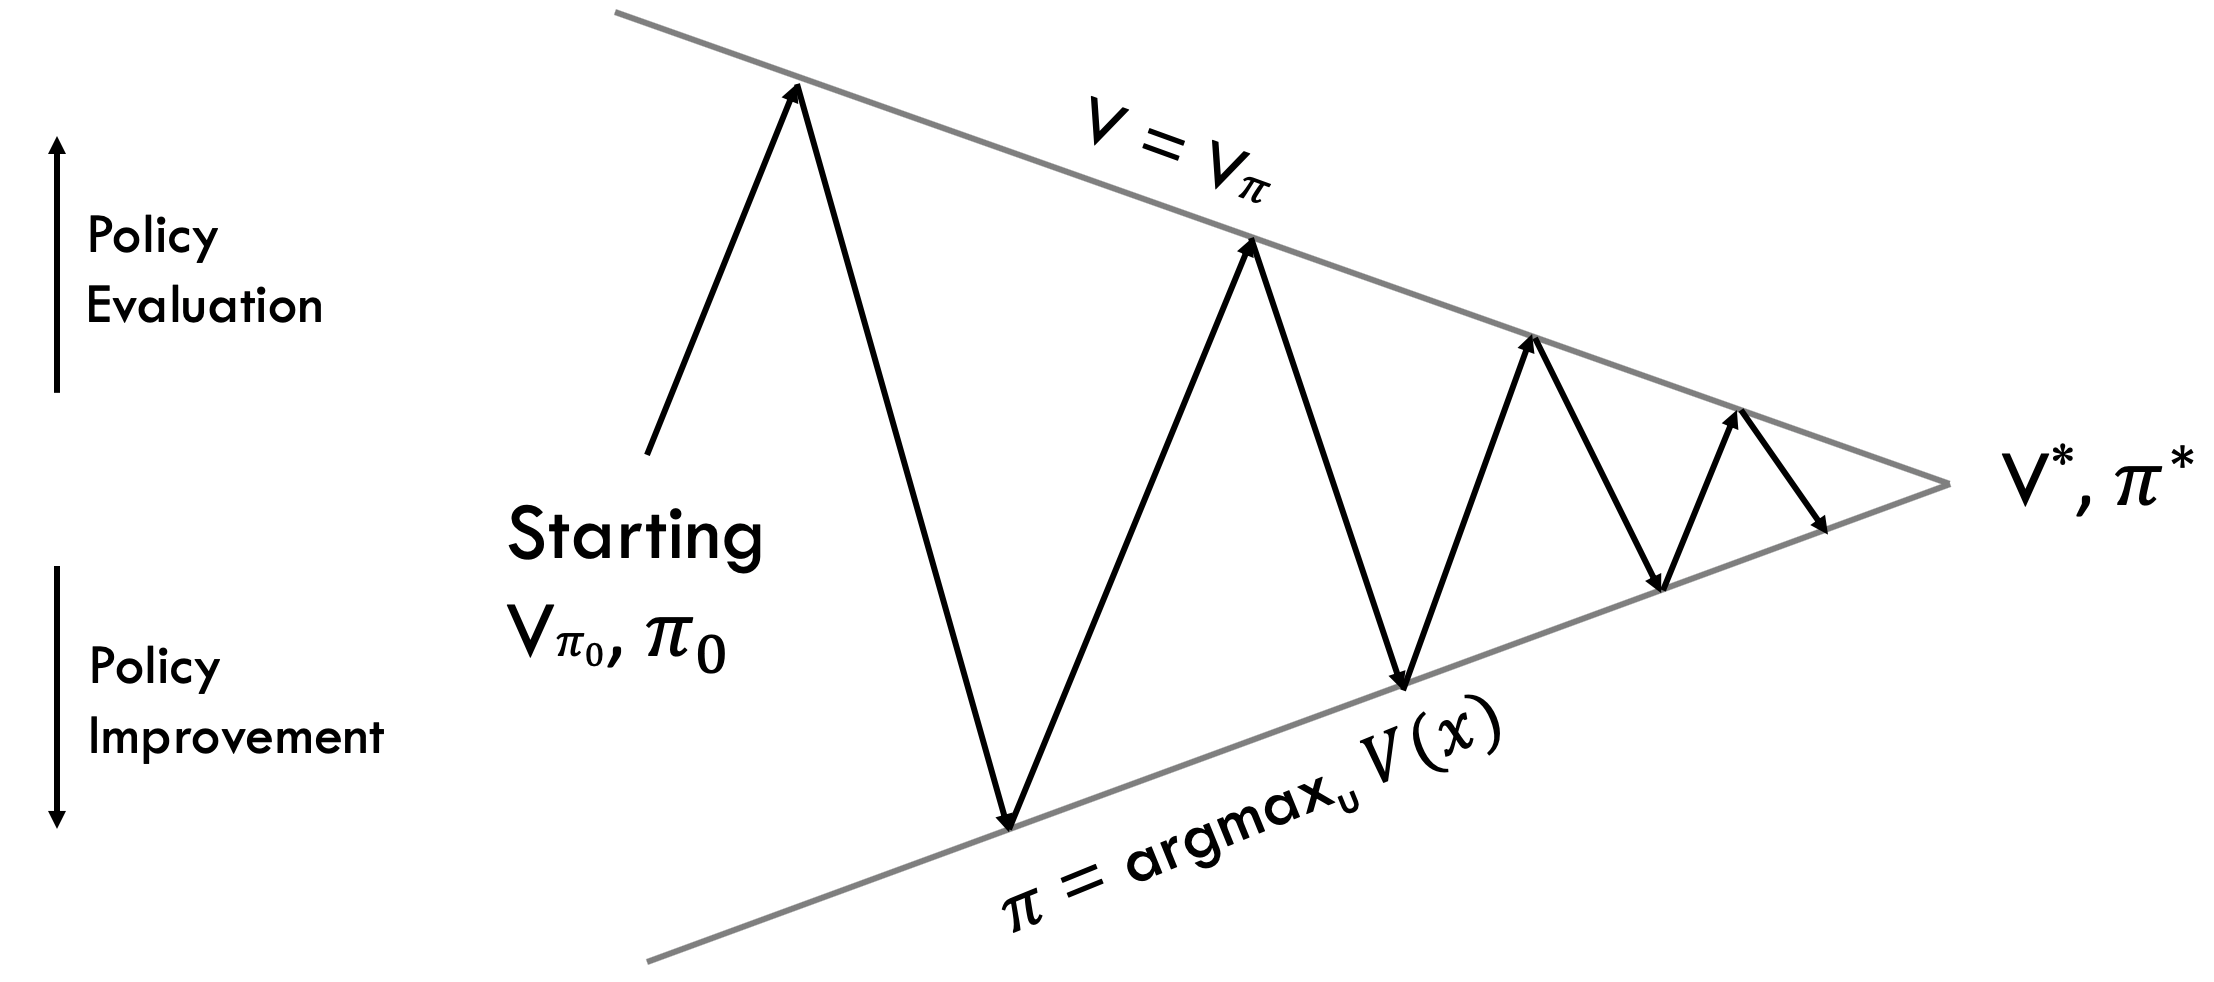
\includegraphics[width=0.68\textwidth]{images/ch1/policy_iteration.jpeg}
    \caption{A visualization of the policy iteration algorithm. Original image from \cite{silver_class}.}
    \label{fig:policy_iteration}
\end{figure}   

To improve upon these computational issues, value iteration was proposed.  Value iteration finds the optimal policy through identifying the optimal value functions instead. Intuitively, value iteration is a special case of policy iteration where the policy evaluation is terminated after one step.  From the value functions of each state, $\pi^*$ can be found by traversing through the states corresponding to the highest values. Note that the optimal policy can only be found using $V(x)$ if a dynamics equation of the system is provided. Without it, $Q(x, u)$ must be identified instead to behave optimally. The policy evaluation for the value iteration algorithm is given as:
\begin{equation}
    v_{k+1}(x) = \max_u \mathbb{E}[R_{t+1} + \gamma v_k(x_{t+1})]
\end{equation}
\begin{equation}
    q_{k+1}(x, u) = \mathbb{E}[R_{t+1} + \gamma \max_{u_{t+1}} q_k(x_{t+1}, u_{t+1})]
\end{equation}
Here, the $max$ operation ensures that each $v_k(x)$ is updated using only the maximizing action so the \textit{optimal} value function can be identified. After all $v^*(x)$ are identified, an agent can behave optimally starting in any state assuming the agent takes the maximizing action at each time. Note that both policy and value iteration are \textit{bootstrap} methods. Bootstrapping in RL increases data efficiency while capturing long-term trajectory information; however, the method also introduces unintended biased. 

In industry, both policy and value iteration have limited utility because their updates are far too computationally expensive. In high dimensional settings, even one iterative step may be intractable; therefore, even with value iteration's reduced computational complexity, it is still infeasible for most complex problems. Asynchronous dynamic programming methods further reduces computational complexity by only updating frequently visited states. However, agents are rendered hopeless in states that are rarely encountered. Although, such a methodology mimics human behaviour where encounters can be handled effectively and efficiently and more exotic situations may catch us by surprise. Nonetheless, such methods still require system models to be explicitly provided, a extremely rare case in industry.

\subsection{Monte Carlo Methods}
Monte Carlo methods no longer require explicit system models (a characteristic known as \textit{model-free}).  Instead, MC methods \textit{estimate} the average returns for different policies through sampling infinitely many sequences of states, actions, and rewards. As the samples increase, $v_k(x) \rightarrow v_{\pi}(x) \text{ for all } x \in \mathcal{X}$. Learning-wise, the average returns are updated at the end of each trajectory. Due to this, the finite tasks with explicit terminal states are typically solved using MC methods. For example, discrete manufacturing is an episodic task in process control. The system is reset after the assembly of each object (cars, toys, ...).  In episodic tasks, the value functions are updated naturally after each episode. However, most tasks in process control are continuous. Training a continuous agent using MC methods require additional modifications. One method is to pre-specify a length of time. After the time has elapsed, the agent will pause and update its value functions. 

Policy search in MC methods is similar to policy iteration. There exists three differences: 1) only visited states are updated; 2) updates use \textit{sampled} data instead of a model; 3) $q_{\pi}(x, u)$ is required and identified instead of $v_{\pi}(x)$. In MC methods, the action-value functions are identified because a model is not provided to the agent. Hence, the agent cannot behave optimally using only the value functions because the actions required to transition to the high value states are not known. Instead, action-values contain explicit information on the expected returns for each action in each state.  The iterative procedure of MC to compute the cumulative returns is given by: 
\begin{equation}
    \pi_0 \xrightarrow{\text{E}} 
    q_{\pi_0} \xrightarrow{\text{I}} 
    \pi_1 \xrightarrow{\text{E}}
    q_{\pi_1} \xrightarrow{\text{I}} 
    \pi_2 \xrightarrow{\text{E}} ... \xrightarrow{\text{I}} 
    \pi^* \xrightarrow{\text{E}}  q_{\pi_*}
\end{equation}
Intuitively, the agent is initiated in an unknown system and follows a certain policy, $\pi$, to traverse throughout the state space while collecting rewards after each decision. Eventually, the agent will reach a terminal state and conclude the episode. Upon termination, a sequence of returns $G_1, G_2, ..., G_{n - 1}$ can be generated using the received reward signals:
$$G_1 = R_{1} + \gamma R_{2} + \gamma^2 R_{3} + ... + \gamma^{n - 1}R_{n}$$
$$G_2 = R_{2} + \gamma R_{3} + \gamma^2 R_{4} + ... + \gamma^{n - 2}R_{n}$$
$$G_3 = R_{3} + \gamma R_{4} + \gamma^2 R_{5} + ... + \gamma^{n - 3}R_{n}$$
$$\vdots$$
$$G_{n - 1} = R_n$$
or:
\begin{equation}
    G_m = \sum\limits_{i=0}^n \gamma^{i} R_{m + i}
\end{equation}
where $G_m$ denotes the discounted cumulative return received on the $m^{th}$ step. Using $G_m$, the action-values can be computed for each step by:
\begin{equation}
    Q_{k+1}(x, u) = Q_{k}(x, u) + \frac{1}{k} \left[G - Q_k(x, u) \right]
    \label{eq:q_update_mc}
\end{equation}
where $Q_k(x, u)$ represents the $k^{th}$ action-value update and $G$ corresponds to the returns received after performing action $u$ in state $x$. Notice that as $k \rightarrow \infty$, $\frac{1}{k} \rightarrow 0$; therefore, this set-up is ineffective in non-stationary settings because the updates get infinitely small.  To extend Equation \ref{eq:q_update_mc} to non-stationary problems, $\frac{1}{k}$ is changed to a constant given by $\alpha$:
\begin{equation}
        Q_{k+1}(x, u) = Q_{k}(x, u) + \alpha \left[G - Q_k(x, u) \right]
        \label{eq:01mcupdate}
\end{equation}
where $\alpha \in (0, 1]$ is known as the learning rate (also called step size). The lower bound prevents $\alpha$ from approaching 0; therefore, allowing for continually adaptation in non-stationary problems. After each update of Equation \ref{eq:01mcupdate}, a new episode starts and the procedures are repeated.  As $k, \text{ \# of episodes } \rightarrow \infty, Q(x, u) \rightarrow q(x, u)$. Once $Q(x, u)$ converge, online action selection can be conducted by:
\begin{equation}
    \pi^*(x) = \argmax_{u} q(x, u)
    \label{eq:policy_extract}
\end{equation}
That is, $\pi^*$ is performing the greedy action in each state.  

\subsubsection{Exploration in MC}
Notice that bootstrapping is not used in MC methods.  In fact, all value functions are estimated independently. As such, MC methods do not suffer from bias issues; however, MC methods may suffer from large variances instead caused by the noise in each sampled trajectory \cite{sutton}. Moreover, exploration is mandatory in MC methods because the dynamics of the system are unknown to the agent. Through exploration, the agent can discover the dynamics of the system and the value functions for each state.  Typically, exploration in MC methods is conducted by initiating the agent in a random state at the beginning of each episode. After infinite episodes, all states will be visited infinitely many times.

MC methods allow the agent to learn solely from sampled data; however, the action-values are updated only after each episode. Such a procedure is unnatural in continuous systems (most systems in process control), disadvantageous long episode systems, and is not intuitive to human behaviour. For example, humans learn immediately after feedback, not in pre-set increments. Temporal difference methods combine the best features of DP and MC methods into one unifying algorithm.





\subsection{Temporal-Difference Methods}
Temporal difference (TD) methods are mathematically simple and cheap computationally compared to MC and DP methods. TD methods learn from experiences (like MC methods) and bootstraps (like DP methods). Furthermore, a dynamics model is not required in TD methods. Instead, the agent learns the dynamics from interactions. Moreover, TD methods update their value functions immediately after $x_{t+1}$ and $R_{t+1}$ are received. The TD update algorithm for value and action-value functions are given in Equations \ref{eq:td_value} and \ref{eq:td_action_value}, respectively \cite{td}:
\begin{equation}
    V(x_t) \leftarrow V(x_t) + \alpha \left[R_{t+1} + \gamma V(x_{t+1}) - V(x_t) \right]
    \label{eq:td_value}
\end{equation}
\begin{equation}
    Q(x_t, u_t) \leftarrow Q(x_t, u_t) + \alpha \left[R_{t+1} + \gamma Q(x_{t+1}, u_{t+1}) - Q(x_t, u_t) \right]
    \label{eq:td_action_value}
\end{equation}
where $\leftarrow$ is the update operator. At each update, the old value function is corrected as a function of the \textit{TD error} by a fixed amount determined by $\alpha$.  The TD errors are at each time $t$ is given as:
\begin{equation}
    \delta_t = R_{t+1} + \gamma V(x_{t+1}) - V(x_t)
    \label{eq:01td_error1}
\end{equation}
\begin{equation}
    \delta_t = R_{t+1} + \gamma Q(x_{t+1}, u_{t+1}) - Q(x_t, u_t)
    \label{eq:01td_error2}
\end{equation}
The first two terms, $R_{t+1} + \gamma V(x_{t+1})$, denote the predicted value function for $x$ in accordance with the last interaction.  $V(x_t)$ is the previously predicted value function for $x$. After infinitely many interactions with the system,  $V(x_t) \rightarrow v(x_t)$ (i.e., the estimated values converge to the true values). The action-values follow the same procedure. After convergence of the values and/or action-values, the optimal action selection is given in Equation \ref{eq:policy_extract}.

\subsubsection{Exploration in TD}
Like MC methods, TD methods are also \textit{model-free}; therefore, action-values are required for the agent to act optimally and exploration is mandatory. A simple and common exploration method used in TD methods is the $\epsilon$-greedy action selection. Here, the agent performs the greedy action with a $\epsilon \in [0, 1]$ probability of performing a random action. During training, $\epsilon$ is typically decayed throughout training.  At the beginning, $\epsilon$ starts at a high value because agent knows nothing. Eventually, $\epsilon$ decays to a low value when training is almost complete. 

Unfortunately, random exploration is sample inefficient and may require the agent to undergo thousands of interactions before learning anything meaningful. Learning can typically be significantly accelerated through a heuristics function $\mathcal{H}: \mathcal{X} \times \mathcal{U} \rightarrow \mathbb{R}$ \cite{harl}.  One such heuristics approach is the upper confidence bound (UCB) action selection algorithm \cite{ucb}. Here, exploration is promoted on states that have high potential to be optimal and is given by:
\begin{equation}
    U_t = \argmax_u [Q_t(x, u) + \mathcal{H}] 
    \label{ucb}
\end{equation}
The heuristics function here is given by:
\begin{equation}
    \mathcal{H} = c \sqrt{\frac{ln \; t}{N_t(x, u)}}
\end{equation}
where $c$ is the degree of exploration.  Large $c$ values promote greater degrees of exploration. Furthermore, $N_t$ is the number of times action $u$ was selected prior to time $t$. As $N_t(x, u) \rightarrow \infty$, the corresponding $Q(x, u)$ has been updated many times and becomes very accurate.  Hence, the heuristics function $\mathcal{H} \rightarrow 0$. 

\subsubsection{Popular TD algorithms}
The two most popular TD algorithms are \textbf{SARSA} and \textbf{$Q$-learning}.  \textbf{SARSA} is an \textit{on-policy} algorithm. In such algorithms, the \textit{behaviour policy} and \textit{target policy} are identical.  Target policy refers to the goal policy of the agent.  Typically, this is the optimal policy.  Conversely, the behaviour policy, $b(u|s)$, is the policy used by the agent for decision making. In cases where the target and behaviour policy are identical, the agent is \textit{on-policy}. One flaw with \textit{on-policy} agents (assuming the target policy is the optimal policy) is that during training, the agent may quickly converge to a local optimum and never explore (since any policies containing exploration is not the optimal policy).  Ultimately, this results in a sub-optimal solution.  Contrarily, \textit{off-policy} agents, like \textbf{$Q$-learning}, typically follow exploratory policies during training to conduct deep exploration.  Then in online applications, the policy is swapped to the optimal policy. Moreover, \textit{off-policy} agents are \textit{guaranteed} to find the optimal policy assuming each state-action pair is visited infinite times and $b(u^* | s) > 0$ (i.e., probability of picking the optimal action under the behaviour policy is not 0) \cite{td}.

Since SARSA is \textit{on-policy}, the action-value function are updated using Equation \ref{eq:td_action_value} using the quintuple $(x_t, u_t, R_{t+1}, x_{t+1}, u_{t+1})$. $Q$-learning updates use only four parameters $(x_t, u_t, R_{t+1}, x_{t+1})$ through Equation \ref{eq:q_learning}:
\begin{equation}
    Q(x_t, u_t) \leftarrow Q(x_t, u_t) + \alpha \left[R_{t+1} + \gamma \argmax_{u_{t+1}} Q(x_{t+1}, u_{t+1}) - Q(x_t, u_t) \right]
    \label{eq:q_learning}
\end{equation}
In $Q$-learning, $u_{t+1}$ is not required because the action taken might follow a different policy compared to the target policy since the algorithm is \textit{off-policy}. Instead, Equation \ref{eq:q_learning} uses the $max$ operation to ensure $Q$-values are still updated towards the optimal policy. Ultimately, TD methods unify DP and MC methods, allowing the agent to learn from experiences and perform inter-episode updates to exploit the most recent learnings.

A detailed numerical example is provided in Chapter 4 where a tabular $Q$-learning algorithm was applied onto an industrial VFD system to conduct set-point tracking control.



\section{Summary of the different solution approaches}
The main features of DP, MC and TD methods are summarized in Table \ref{tab:dc_mc_td}. Overall, DP requires a dynamics function of the system to compute the value functions while both MC and TD methods can learn directly from interactions with the system. Both DP and TD methods use bootstrapping to estimate value functions, that is, they estimate the current value function based on previously estimated values. Bootstrapping is data efficient, but introduces large bias to the estimated values, especially in the early episodes.  Conversely, MC methods estimate the value functions of each state independently through sampling many system trajectories.  However, this method, instead, introduces high variance. For extremely noisy systems, the reproducability of the results may be difficult. Comparing the computational cost, DP methods require much more compared to MC or TD since all value functions are simultaneously solved. In MC methods, only the value functions that were visited in the sampled trajectories are updated.  Additionally, updates are conducted at the end of each episode and not after each step. Similar to DP methods, TD methods update the value function immediately after an experience; however, only the value function corresponding to the last visited state is updated. In terms of exploration, DP methods do not explore the system model (both transition probabilities and expected reward) is explicitly provided. MC methods explore by being initiated in a random state after each episode termination. In TD methods, agents explore by occasionally performing a random action.

\begin{table}[H]
\caption{A comparison of DP, MC, and TD methods.}
\label{tab:dc_mc_td}
\centering
{\scriptsize
\begin{tabular}{c|c|c|c}
 & \textbf{Dynamic Programming}	& \textbf{Monte Carlo} & \textbf{Temporal Difference}\\
\hline
Requires model	     	& Yes			& No     &  No \\
Estimate bias           & High			& Low    &  High \\
Estimate variance	    & Low			& High   &  Low \\
Computational cost		& High			& Medium &  Low \\
$v(x)$ update      	& All states simultaneously   & After a trajectory  &  After an experience \\
Exploration             & Not needed, all states update   & Random initialization  &  Performing a random action \\
\end{tabular}}
\end{table}




\section{Reward design for process control}
The design of the reward function for process control applications is similar to MPC.  For regulation or set-point tracking problems, the MSE reward function can be used and is given by:
\begin{equation}
    r(x, u) = -(x_i - x_{sp})^2
\end{equation}
However, the agent may find it difficult to distinguish between small off-sets using this reward function.  For example, when the tracking error is 10, the reward is -100.  However, if the off-set is only 0.25 or 0.1, the agent would find it difficult to distinguish between the small rewards because the difference is miniscule compared to an error of 10.  To enhance this distinction, a Huber loss can be used \cite{huber}:
\begin{equation*}
    r(x, u) = \begin{cases}
    x_t - x_{sp} & \quad if \; |x_t - x_{sp}| > 1 \\
    (x_t - x_{sp})^2 & \quad otherwise
    \end{cases}
\end{equation*}
In this case, large errors are not squared, significantly reduce their magnitude.  In the tabular cases, this error works exceptionally well; however, not so much in deep RL.  Typically, the inputs to neural networks are normalized for sufficient learning \cite{NN}.  When normalizing the rewards, small errors will once again become indistinguishable.  In such a case, the following reward function typically works better:
\begin{equation*}
    r(x, u) = \begin{cases}
    x_t - x_{sp} & \quad if \; |x_t - x_{sp}| > 1, \\
    (x_t - x_{sp})^2 & \quad if \; 1 \geq |x_t - x_{sp}| > \eta, \\
    +1 & \quad otherwise
    \end{cases}
\end{equation*}
where $\eta$ is the maximum acceptable tracking error. Here, as the agent achieves states within $\eta$, the rewards are significantly increased.  Such an idea is similar to zone MPC, where the objective of the controller is to guide the trajectory within a zone \cite{zone_mpc}. Another flaw with deep RL comes from the noisy action signals.  For example, a normal human would not go and continuously change the air conditioning set-point if the temperature inside a house varies between $\ang{22.1}$ C to $\ang{22.2}$ C because the two temperatures are relatively the same.  In the case of deep RL, these are seen as two completely different states, and correspond to (slightly) different actions.  One could design a filter to remove such small actions from being sent to the system; however, adding a cost to the change in inputs is a more natural way to mitigate this:
\begin{equation}
    r(x, u) = -[(x_t - x_{sp})^2 + \nu \Delta u_t^2]
\end{equation}
where $\Delta u_t$ is the change in input in the last sampling time. The coefficient, $\nu$, is used to tune the effect of the action on the reward.  For example, if the system's input signals are typically small, a large $\nu$ would be used so the tracking error does not dominate the entire reward function.

In exotic scenarios where the optimal input is known, the reward function can become:
\begin{equation}
    r(x, u) = -[(x_i - x_{sp})^2 + (u_i + u_{ss})^2]
\end{equation}
Lastly, the rewards are sometimes clipped to avoid large TD errors causing numerical issues during bootstrapping \cite{reward_clip}.  From Equation \ref{eq:q_learning}, it can be seen that if $R(x, u) >>> Q(x, u), Q(x_{t+1}, u_{t+1})$, then the updated $Q(x, u)$ would be completely dominated by $R(x, u)$. Additionally, any future updates bootstrapping off $Q(x, u)$ would subsequently become dominated by its value. As such, rewards are clipped (bounded) within a range to prevent such issues. Unexpectedly large rewards may originate from incorrect sensor readings, which consequently leads to inaccurate reward signals being sent to the agent.  Reward clipping is conducted by:
\begin{equation}
    r(x, u) = min(max(r_t,\mu^- ), \mu^+)
    \label{reward_clipping}
\end{equation}
where $\mu^-$ and $\mu^+$ denotes the minimum and maximum rewards, respectively. 




\subsection{Reinforcement Learning vs. Other "Learnings"}

Reinforcement learning is a unique class of machine learning.  An ideal supervised learning model can only be as good as the subject matter expert providing the labels to the data set, which may not be 100\%.  For example, in a complex control task, the control law is usually highly non-linear. Control experts can try to provide control strategies for such systems, but optimality may not be guaranteed for highly non-linear systems. Also, supervised learning is used to generalize responses for occurrences not present in the data \cite{sutton}.  Reinforcement learning works by directly interacting with the environment \textit{without labels}. Through adequate exploration, reinforcement learning will identify peculiar features to optimally control such problems [citation required].  Reinforcement learning is \textit{similar} to unsupervised learning in terms of identifying hidden structures within the environment.  However, reinforcement learning tries to maximize an internal scalar "reward" signal, rather than purely data mining.

Evolutionary methods, a family of optimization algorithms such as genetic algorithm, are most similar to reinforcement learning.  For a control problem, such methods can apply multiple static policies for different operating regimes \cite{sutton}.  Policy search is conducted by first initiating $k$ random input trajectories of length $N$, generating input matrix $\mathbb{U}_{[k, N]} \in \pi$.  Subsequently, the loss, $J_U$, of each $U$ is calculated based on the objective function.  Input trajectories with the lowest loss move onto the next generation and generates new pseudo-random input trajectories.  This process is repeated until optimal policy, $\pi^*$ is found for each operating regime \cite{ga_for_control}.

Evolutionary methods work well when the policy space is sufficiently small, easy to find, or a lot of time is available for optimization.  The biggest advantage of such methods compared to reinforcement learning is that the whole state does not need to be known.  However, such methods does not capture the reinforcement learning fundamentals of mapping $X \rightarrow U$.  Unlike evolutionary methods, reinforcement learning keeps memory of each individual interaction making it a more data efficient approach \cite{sutton}.

%%%%%%%%%%%%%%%%%%%%%%%%%%%%% End Section Intro to RL %%%%%%%%%%%%%%%%%%%%%%%%%%%%%%%%%%%%%%%



%%%%%%%%%%%%%%%%%%%%%%% Begin Section Function Approximation %%%%%%%%%%%%%%%%%%%%%%%%%%%%%%%

\section{Function Approximation}
\subsection{Introduction to Function Approximations}
Prediction models have wide applications in all sectors of the economy.  To obtain the highest possible accuracy, one can simply have an infinitely large repository of previous examples.  When given any input, a suitable output can be generated by finding the exact solution in the repository.  For example, if the task is to predict the model of an automobile based on a picture and the dimensions of a car, one could obtain 100\% accuracy so long as every single car specification exists in a repository.  This idea sounds good in theory, but is only possible in real life if there exists infinite memory.  Function approximation aims to solve this problem by generating a model to generalize across a massively large repository of historical data.  Intuitively, the model stores the information at a much lower space complexity, for a cost of some reproduction error.  There is also a trade-off between the reduced space complexity and the reproduction error.  Large, complex models have increased space complexity but reduced error while small, simple models exhibit the opposite.  This section focuses on complex neural network models with high predictive capabilities.  In RL, function approximation is typically used to approximate the (action-) value functions or the policy itself.


\subsection{Neural Network Basics}
Neural networks are highly non-linear models that explore the individual and interaction effects of each variable with all other variables \cite{NN}. The general structure of a neural network is shown in Figure \ref{fig:08NN}.  Neural networks are comprised of an input layer, some hidden layer(s), and an output layer.  The input layer consists of the input data, while the hidden layer(s) and output layer consists of fitted weights and biases, $W_{n_x \times n_b}$ and $b_{n_b \times 1}$, respectively. Here, $n_b$ and $n_x$ denotes the batch size and the dimension of the input layer, respectively. In Figure \ref{fig:08NN}, $x_m$ denotes the $m^{th}$ input variable.  The superscript and subscript of $a$ denotes the hidden layer number and the node number in the corresponding layer, respectively.  Subscript $m_1$ to $m_r$ denotes the number of nodes in hidden layers 1 to $r$, respectively.  Finally, superscript $o$ denotes the output layer.
\begin{figure}[h]
    \centering
    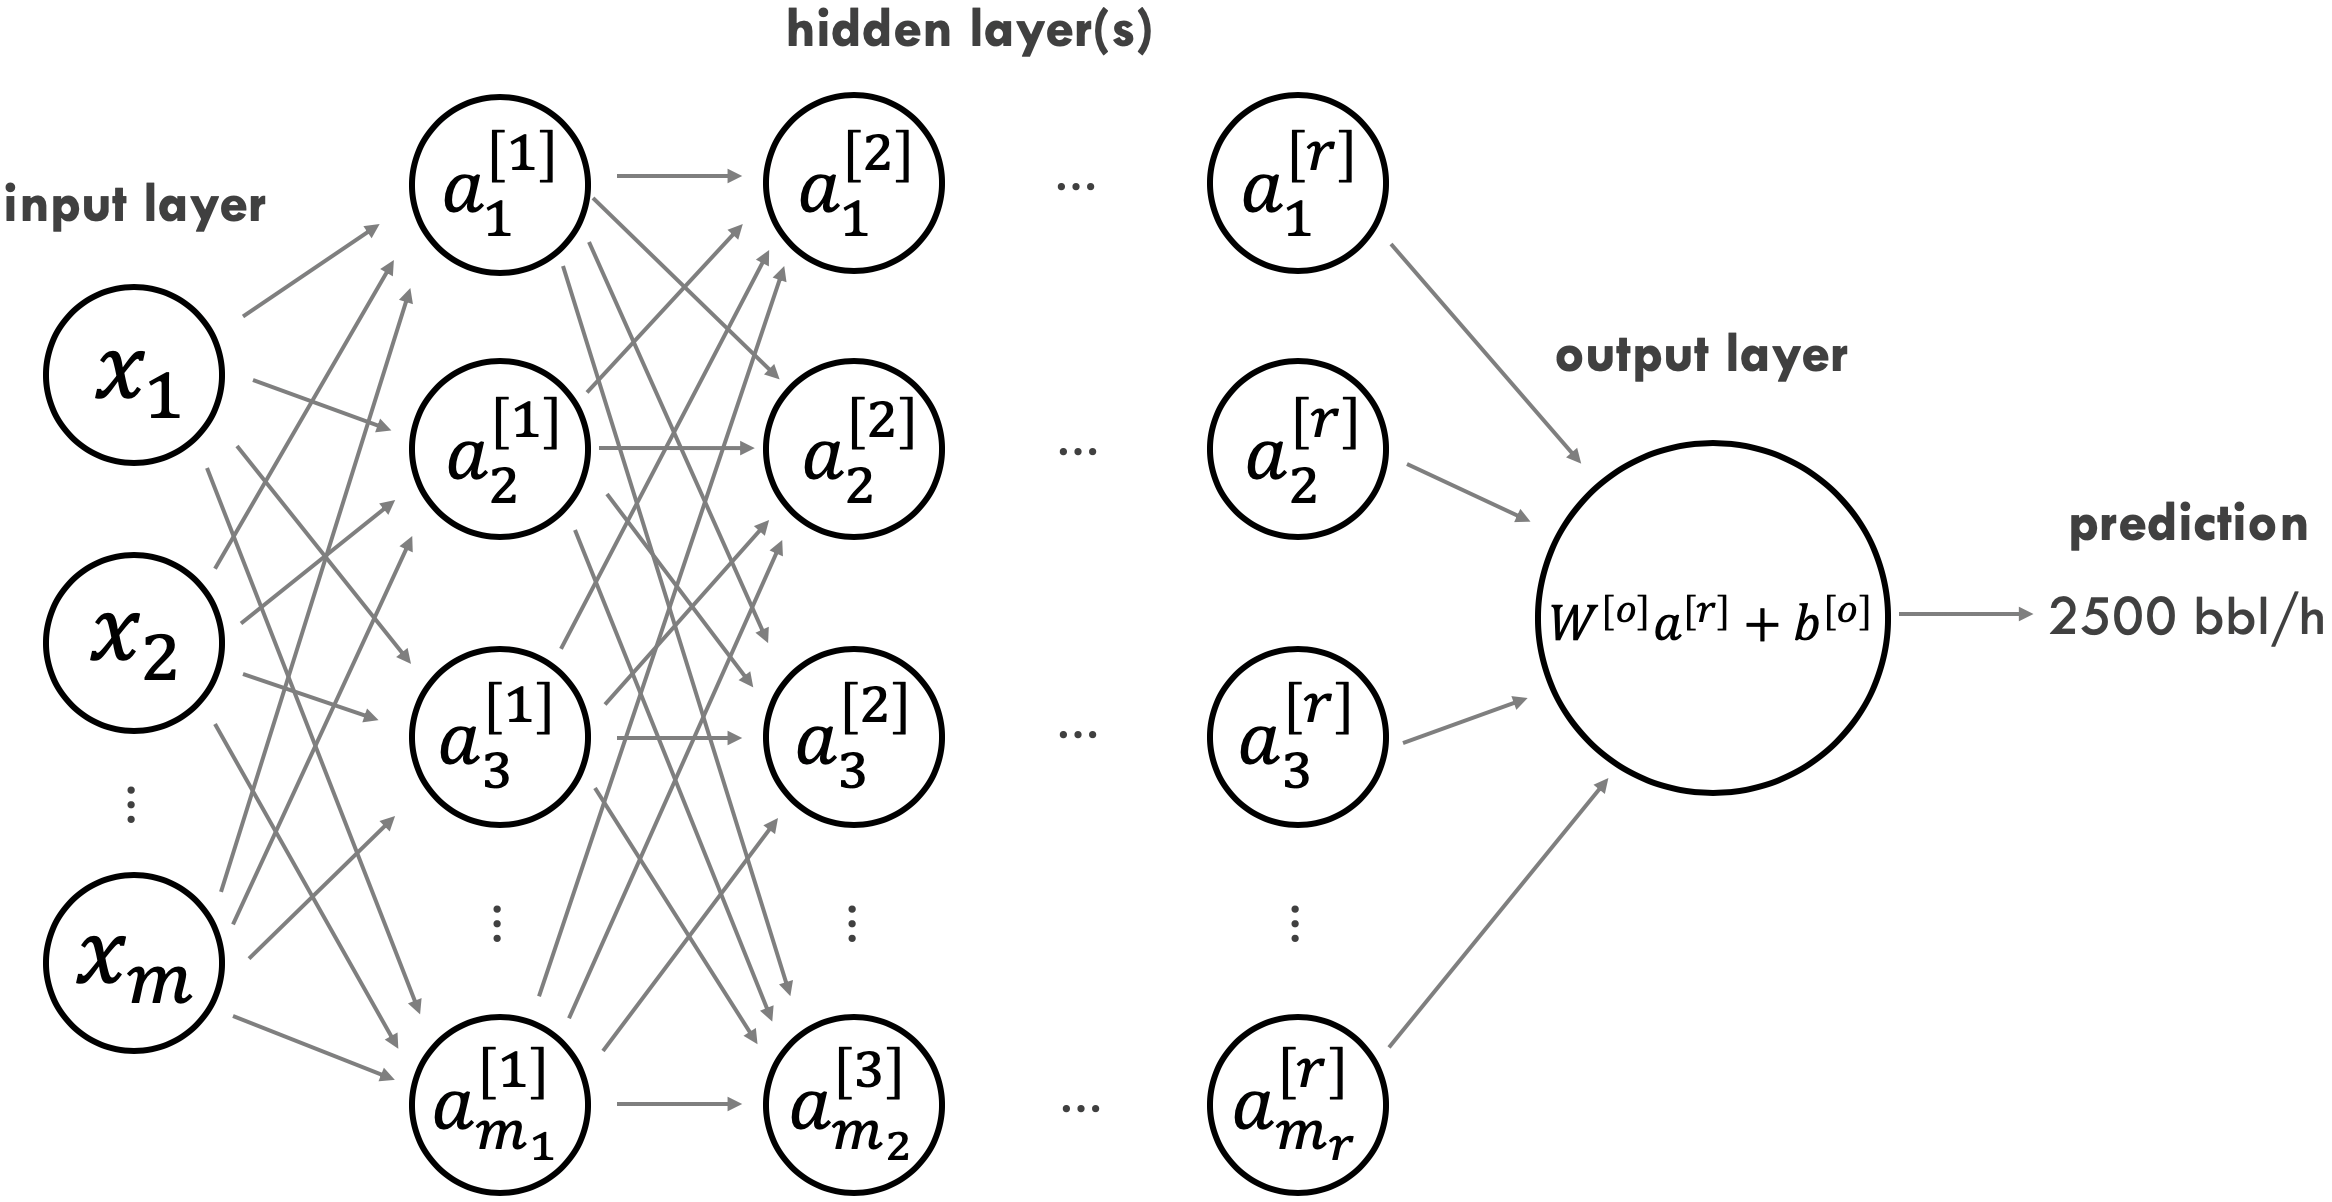
\includegraphics[width=0.9\textwidth]{images/ch1/08NN.png}
    \caption{Structure of a general neural network.}
    \label{fig:08NN}
\end{figure}


The details within a hidden layer's node is shown in Figure \ref{fig:08NNNode}. First, the outputs from the previous layer's nodes are inputted and multiplied by the weights of the current node.  The current node's bias is then added. If the current node is in the first layer, the outputs from the previous layer is replaced with the input variables. Afterwards, the output is sent to an action function to provide the non-linearity for any neural network model.  In this thesis, the rectified linear unit (ReLU) activation function is typically used and is given by:
\begin{equation}
    a^{[i]}_j=\begin{cases}
        y, & \text{if $y\geq0$}.\\
        0, & \text{otherwise}.
    \end{cases}
    \label{eq:08ReLU}
\end{equation}
where $i$ and $j$ denotes any hidden layer and any node number, respectively.  Two other popular activation functions are sigmoid and tanh given in Equations \ref{eq:01sigmoid} and \ref{eq:01tanh}, respectively.
\begin{equation}
    a^{[i]}_j = \frac{1}{1 + e^{-z}}
    \label{eq:01sigmoid}
\end{equation}
\begin{equation}
    a^{[i]}_j = \frac{e^z - e^{-z}}{e^z + e^{-z}}
    \label{eq:01tanh}
\end{equation}
where $e$ denotes the exponential operator and $z = Wx + b$. The sigmoid and tanh activation functions have lost popularity in recent years because they create the exploding/vanishing gradient effect.  This effect occurs because the derivatives of both the sigmoid and tanh functions are zero outside of a small section.  Additionally, the derivative at the inflection point is infinity.  Since neural networks are trained using backpropagation, often times, the gradient of the loss function becomes zero as it is backpropagated through the neural network during training.  Ultimately, this leads to significant difficulties in training neural networks (especially deep networks) \cite{vanish_grad}.  

\begin{figure}[h]
    \centering
    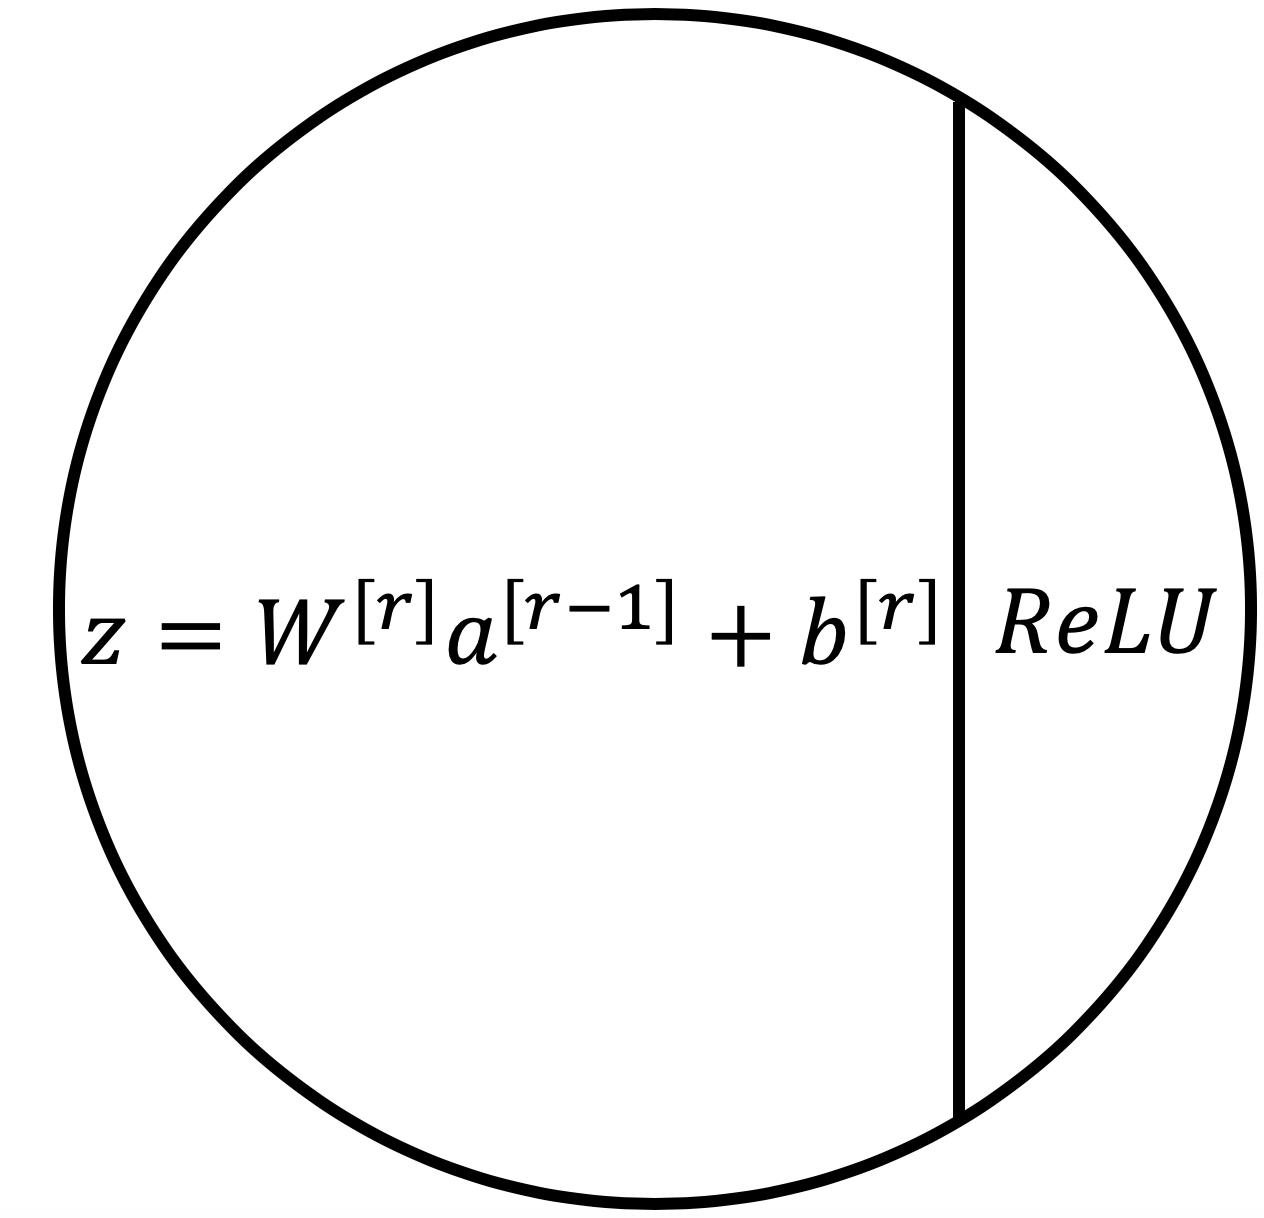
\includegraphics[width=0.3\textwidth]{images/ch1/08NNNode.png}
    \caption{Inside a hidden layer's node.}
    \label{fig:08NNNode}
\end{figure}

Mathematically, for one example with input vector $x$:
\begin{center}
    $z^{[1]}_j = W^{[1]}x + b^{[1]}$ \\
    $a^{[1]}_j = ReLU(z^{[1]}_j)$ \\
    $z^{[2]}_j = W^{[2]}a^{[1]}_j + b^{[2]}$ \\
    $a^{[2]}_j = ReLU(z^{[2]}_j)$ \\
    ... \\
    $z^{[r]}_j = W^{[r]}a^{[r - 1]}_j + b^{[r]}$ \\
    $a^{[r]}_j = ReLU(z^{[r]}_j)$ \\
    $y = W^{[o]}a^{[r]}_j + b^{[o]}$ \\  
\end{center}




\subsubsection{Neural Network Initialization}
Neural networks can be initiated in many ways. Although neural networks can be initiated as all zeros, such an approach is not symmetry-breaking resulting in all neurons performing the same calculations \cite{NN}.  Ultimately, this results in all neurons outputting the same values rendering the whole network useless.  Therefore, a primitive approach to overcome this was to initialize the neural network weights as random near-zero values. This method was symmetry-breaking, but such networks required long training times, especially in deep learning \cite{xavier_init}. In 2010, Xavier and Bengio published one of the first papers to explicitly study neural network initialization.

In \cite{xavier_init}, the the Xavier initializer was proposed to equalize the variance of the outputs of each layer with the variance of its inputs. More specifically, the biases of each layer was initialized as zero, but the weights were initialized as:
\begin{equation}
    W \thicksim U \left[-\frac{\sqrt{6}}{\sqrt{n_j + n_{j+1}}}, \frac{\sqrt{6}}{\sqrt{n_j + n_{j+1}}}  \right]
    \label{eq:01xavier}
\end{equation}
where $U[-a, a]$ represents an uniform distribution bounded between $(-a, a)$.  Here, $n_j$ and $n_{j+1}$ denotes the size of the previous and current layers. The derivation of Equation \ref{eq:01xavier} assumed linear actions. When tested using sigmoid activation functions, the Xavier initialized neural networks showed substantially faster convergence times. Unfortunately, sigmoid activation functions were considered obsolete as time went on due to the exploding/vanishing gradients problem \cite{vanish_grad}.  

By 2015, He et al. proposed a new initialization method specialized for ReLU activation functions, known as the He initializer \cite{he_init}. He extended upon previous work by assuming a ReLU activation function instead of a linear one and obtained the weight initialization function given by:
\begin{equation}
    W \thicksim \mathcal{N} \left(0, \frac{2}{n_j}  \right)
\end{equation}
where $\mathcal{N}$ denotes the Gaussian distribution and $\frac{2}{n_j}$ denotes its standard deviation.  Like in \cite{xavier_init}, the He initialization showed substantially faster convergence times for neural networks compared to previous methods when using the ReLU activation function.

The advantages of each initialization are summarized in Table \ref{tab:01nn_init}

\begin{table}[H]
\caption{Comparing different neural network initialization methods.}
\label{tab:01nn_init}
\centering
{\footnotesize
\begin{tabular}{c|c|c|c}
\textbf{Zero init.} & \textbf{Random init.}	& \textbf{Xavier init.} & \textbf{He init.}\\
\hline
Does not work	     	& Simple but slow			& Ideal for sigmoid activations &  Ideal for ReLU activations \\
\end{tabular}}
\end{table}




\subsection{Cost function for neural networks}
MSE is the typical cost function for regression tasks and is given by \cite{NN}:
\begin{equation}
    J(\theta) = \frac{1}{n}\sum\limits^n_{i=1}(\hat{y}_i - y_i)^2
    \label{eq:08MSE}
\end{equation}
where $J$ represents the loss.  Here, $n$ denotes the number of samples in the current optimization step. $\hat{y}_i$ and $y_i$ are the $i^{th}$ predicted and actual labels, respectively. The MSE cost function is typically selected due to its convex nature \cite{deeplearning_course}.


\subsubsection{Gradient descent}
Given the cost function, the model parameters are updated using gradient descent. The general gradient descent formulation is given by Equation \ref{eq:08GradientDescent}.  
\begin{equation}
    \theta_j^{m+1} \leftarrow \theta_j^{m} - \alpha \frac{\partial J}{\partial \theta_j}
    \label{eq:08GradientDescent}
\end{equation}
where $\theta_j$ denotes the $j^{th}$ parameter (parameter includes both weights and biases) of the model.  Here, $m$ represents the $m^{th}$ update of gradient descent and $\alpha$ is the learning rate. Unfortunately, gradient descent can optimize quite slowly, especially for neural networks where the solution is highly non-convex. There are many different enhanced gradient optimization methods such as momentum gradient descent, AdaGrad, RMSprop, etc; however, adaptive momentum gradient descent (ADAM) method will be used for the remainder of this thesis \cite{ADAM}. Mathematically, ADAM combines momentum gradient descent and RMSprop into one unifying algorithm. ADAM improves upon Equation \ref{eq:08GradientDescent} by computing an adaptive learning rate for each parameter \cite{ADAM}. To do so, the exponentially decaying average of the past gradients and squared gradients of the weights and biases are computed and stored using Equations \ref{eq:08momentW} to \ref{eq:08squared_momentb}.
\begin{equation}
    V_{dW} = \beta_1 V_{dW} + (1 - \beta_1)dW
    \label{eq:08momentW}
\end{equation}
\begin{equation}
    V_{db} = \beta_1 V_{db} + (1 - \beta_1)db
    \label{eq:08momentb}
\end{equation}
\begin{equation}
    S_{dW} = \beta_2 S_{dW} + (1 - \beta_2)dW^2
    \label{eq:08squared_momentW}
\end{equation}
\begin{equation}
    S_{db} = \beta_2 S_{db} + (1 - \beta_2)db^2
    \label{eq:08squared_momentb}
\end{equation}
where $V$ and $S$ are the estimates of the gradient and squared gradients, respectively.  $V$ and $S$ are typically initiated as zero vectors and are heavily biased towards zero at initial steps.  Hence, the biases (numerical bias, not the neural network parameter bias) for the initial terms are corrected using:
\begin{equation}
    V_{dW}^{corrected} = \frac{V_{dW}}{1 - \beta_1^t}
\end{equation}
\begin{equation}
    V_{db}^{corrected} = \frac{V_{db}}{1 - \beta_1^t}
\end{equation}
\begin{equation}
    S_{dW}^{corrected} = \frac{S_{dW}}{1 - \beta_2^t}
\end{equation}
\begin{equation}
    S_{db}^{corrected} = \frac{S_{db}}{1 - \beta_2^t}
\end{equation}
Combining the above equations, the weights and biases are updated by:
\begin{equation}
    W_j \leftarrow W_j - \alpha \frac{V_{dW}^{corrected}}{S_{dW}^{corrected} + \epsilon}
\end{equation}
\begin{equation}
    b \leftarrow b - \alpha \frac{V_{db}^{corrected}}{S_{db}^{corrected} + \epsilon}
\end{equation}
where $\epsilon$ is a small scalar to avoid division by zero. The authors proposed values of 0.9, 0.999 and $10^{-8}$ for $\beta_1$, $\beta_2$, and $\epsilon$, respectively \cite{ADAM}.  Next, the amount of data that will be used to compute the loss gradient will be explored.

\subsubsection{Mini-batch gradient descent}
Classically, the gradient of the loss function was computed using all data available. Furthermore, this method (called batch gradient descent) guarantees monotonic improvements in performance after each update step \cite{deeplearning_course}. However, BGD suffers from space complexity and is infeasible in big data applications.  Thus, mini-batch gradient descent was used for the work in this thesis. Mini-batch gradient descent fits between stochastic gradient descent (SGD) and BGD, where small batches of data sampled from the original data set are used to perform stochastic updates at each step \cite{sgd}. Mini-batch gradient descent offers three benefits over the previous methods: i) less computationally demanding compared to batch gradient descent; ii) more accurate loss function gradient for parameter updates compared to SGD; iii) requires less steps compared to SGD.



\subsubsection{Data segregation}
The data set was split into three sections for machine learning: training, validation, and testing.  The partition and description of each section is shown in Table \ref{tab:08datapart}. The training data set was used to identify the machine learning model(s).  Then, the model was validated on unseen data via the validation data set (sometimes called development data).  The error of the model on the validation data set, $e_{validation}$, was then evaluated and compared to the training data error, $e_{train}$.  If the difference is large, the model was rebuilt using different data pre-processing techniques and features. This step was repeated until $e_{train} \approx e_{validation}$ to ensure that the model did not overfit to the training data. Finally, the model was tested on the testing data to explore the performance of the model in live production.  Testing data was always the last 5\% of the data set.
\begin{table}[h]
    \centering
    {\setstretch{1.2}
    \begin{tabular}{ c | c | p{9cm}}
                            & \% of Data        &  Description \\
        \hline
        Training            &  90\%             
        &  Identify the ML model        \\
        
        Validation          &  5\%              
        &  Tune ML model performance on unseen data         \\
        
        Testing             &  5\%             
        &  Test ML model performance on proxy live data       \\     
    \end{tabular}}
    \caption{Description of each data partition.}
    \label{tab:08datapart}
\end{table}
\subsubsection{Regularization}
Objectively, supervised learning models attempt to generalize the learnings obtained from the training data set to predict for situations not seen before. For example, suppose there exists a data set that contains the height and weight of a species of dogs. Objectively, the model must predict the weight of the dog given its height.  After the model is trained, it should have sufficient capability to predict for the weight of a dog even if the exact height provided was not in the training data set.  Often times, the training data set is small and does not represent the whole population of the data set.  This ultimately leads to the model overfitting the training data set, resulting in poor generalization characteristics. In machine learning literature, the model error is often called the \textbf{bias}.  Similarily, the difference in the modelling error between the training and validation data set is called the \textbf{variance} \cite{NN}.  Models exhibiting high variance are typically overfit to the training data, and does not predict well in production.  Regularization aims to significantly reduce variance at only a slight cost to bias. Generally speaking, regularization reduces the likelihood of learning a complex model by penalizing large weights through the objective function.  One common method is called the L1 regularization (sometimes called Lasso regularization) where a linear penalty is applied to weights and is given by:
\begin{equation}
    J(W) = \frac{1}{n} \left[\sum\limits^n_{i=1}(\hat{y}_i - y_i)^2 + \lambda \sum\limits^p_{j=1} |W_j| \right]
    \label{eq:01L1}
\end{equation}
where $\lambda$ is a hyper parameter to determine the aggressiveness of the penalty and $p$ denotes the number of parameters inside the model. The L2 regularization is another popular regularization technique and applies a quadratic instead:
\begin{equation}
    J(W) = \frac{1}{n} \left[\sum\limits^n_{i=1}(\hat{y}_i - y_i)^2 + \lambda \sum\limits^p_{j=1} W_j^2 \right]
    \label{eq:01L2}
\end{equation}
Figure \ref{fig:01l1vsl2} shows the optimal solution space of the L1 and L2 regularizations for a two parameter model. Overall, L2 regularization is typically the preferred choice because of its unique, stable solution and invariance under rotation \cite{l1_l2}. Another key difference is that L1 regularizations cannot be used for gradient based approaches because it is not continuously differentiable \cite{l1_diff}. 

\begin{figure}[H]
    \centering
    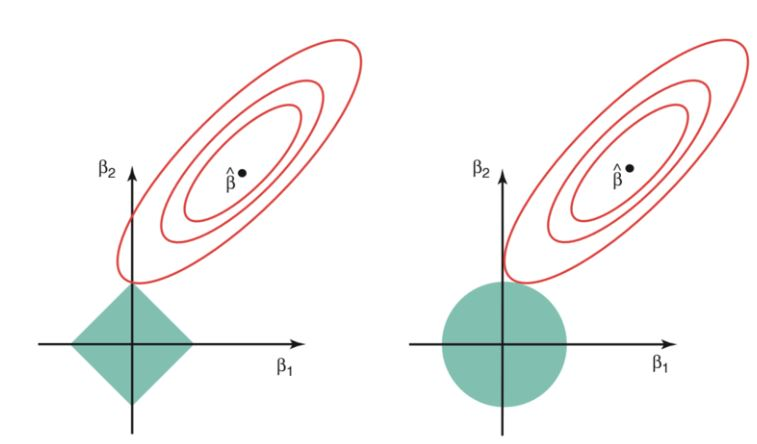
\includegraphics[width=0.56\textwidth]{images/ch1/L1_vs_L2.JPG}
    \caption{Solution space of the lasso (left) and ridge regularization (right). Original image from \cite{generic_stats}.}
    \label{fig:01l1vsl2}
\end{figure}   

Two other popular, but specialized regularization techniques catered towards neural networks are drop-out and batch normalization \cite{dropout, batch_norm}. Figure \ref{fig:01dropout} shows a neural network with and without drop-out. On a high level, drop out randomly disable neurons during training to prevent major "co-adaptation" between adjacent neurons. Intuitively, the drop-out process introduces (significant) pseudo noise into the training step, forcing neurons to learn a more probabilistic mapping. Ultimately, the drop-out method was able to achieve state-of-the-art performance when tested on various data sets in computer vision, natural language processing, classification, and computational biology. A more detailed explanation of drop-out can be found in \cite{dropout}.   

\begin{figure}[H]
    \centering
    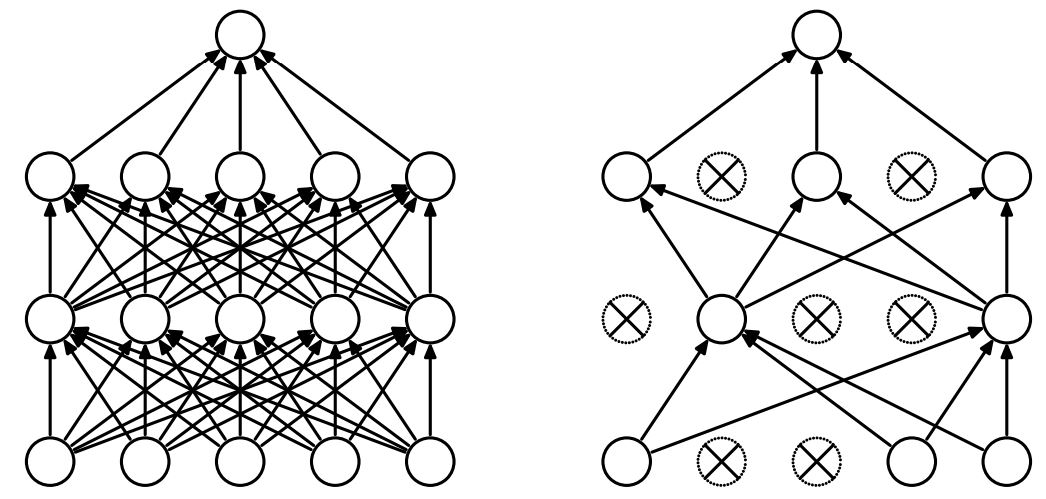
\includegraphics[width=0.56\textwidth]{images/ch1/dropout.jpg}
    \caption{A neural network with (right) and without (left) drop-out \cite{dropout}.}
    \label{fig:01dropout}
\end{figure}  

Batch normalization is another recently popularized regularization method in deep learning.  Neural networks are trained through backpropagation.  In this method, the accuracy of the neurons in the later layers are paramount for proper parameter updates in the earlier layers.  If not, the backpropagated errors are significant incorrect. Specifically, the distribution of different layer's inputs change during training due to the weight changes of the subsequent layers. This characteristic, called internal covariate shift, contains a significantly negative effect on the training time of neural networks.  Batch normalization aims to overcome internal covariate shift by normalizing layer inputs.  In doing so, deep neural networks are less sensitive to initializations and much larger learning rates can be used. Additionally, the method was shown to contain regularization effects and often times eliminate the need for drop-out.  In experiments, the authors found that neural networks using batch normalization can achieve previous accuracies with 14 times fewer training steps.  For more information on batch normalization, see \cite{batch_norm}.


%%%%%%%%%%%%%%%%%%%%%%%%% End Section Function Approximation %%%%%%%%%%%%%%%%%%%%%%%%%%%%%%%


%%%%%%%%%%%%%%%%%%%%%%%%%%%%%%%%% Begin Section DDPG %%%%%%%%%%%%%%%%%%%%%%%%%%%%%%%%%%%%%%%

\section{Deep Deterministic Policy Gradient}
Deep deterministic policy gradient was introduced as one of the first RL architectures to handle both continuous states and continuous actions \cite{ddpg}. Additionally, it was shown to also work in massively large state and action space systems (one such system was $x \in R^{102}$ and $u \in R^{9}$). DDPG contains four neural networks and employs an actor-critic framework.  The actor is the deterministic policy gradient (DPG) algorithm and maps states to actions.  Similarily, the critic is the deep $Q$-learning network (DQN) algorithm and approximates the action-values of the state-action pairs. Intuitively, combining DPG and DQN into one unifying algorithm overcomes several shortcomings exhibited by each algorithm individual. For example, policy gradients were traditionally trained using MC methods and cannot update mid-episode; however, DDPG trains the DPG using the gradient of the DQN, allowing for inter-episode updates. Furthermore, DQN cannot output continuous actions, but DDPG can by leveraging DPG to select actions.  Another advantage provided by DDPG is the mitigation of large variances in the DPG through the use of DQN.  Previously, DPG experiences high variance because similar action sequences may return different outcomes in stochastic environments; however, evaluating the action using the DQN (a deterministic function) will result in an unbiased estimate of performance \cite{ddpg}.  

\subsection{Actor - Deterministic Policy Gradient}
The DDPG leverages the DPG algorithm to deterministically map \textit{continuous} states to \textit{continuous} control actions.  Classically, policy gradient algorithms represent the policy as a probability distribution $\pi_{\theta}(u|x) = \mathbb{P}[u|x; \theta]$ which stochastically maps states to actions \cite{dpg}.  In DPG, \textit{deterministic} policies are considered instead and are given by $u = \mu_{\theta}(x)$. Comparatively, deterministic policies are more advantageous because only $Q^{\mu}(x, \mu_{\theta}(x))$ is required during updates steps compared to $\sum\limits_u \pi(u|x)Q^{\mu}(x, u)$. Here, $\pi(u|x)$ denotes the probabilities of picking different actions $u$ in $x$.

Like all experience driven RL algorithms, exploration is required in DPG; thus, requiring some stochastic behaviour policy (ironically making it non-deterministic). To this end, DPG can be trained using an \textit{off-policy} actor-critic method where a deterministic policy is identified while following a separate exploratory policy.  Such a concept is analogous to $Q$-learning, where a deterministic greedy policy is identified while following a noisy behaviour policy (typically $\epsilon$-greedy) during training. For a detailed explanation of DPG, please refer to \cite{dpg}.


\subsection{Critic - Deep Q-learning Network}
In DDPG, DQN is used to reduce variance and provide off-policy training to the DPG. DQN is a deep $Q$-learning approach to map from states to action-value functions \cite{dqn1, dqn2}. Historical methods to train deep $Q$-learning were unstable and data inefficient. Authors of DQN introduced two important concepts in the DQN algorithm---the experience replay and target networks---to significantly improve convergence rate. The \textit{experience replay} is a dictionary of tuples $(x, u, r, x')$.  During training, random mini-batch of experience tuples are sampled to enhance data efficiency (same experiences used many times) and to provide the agent with temporally de-correlated training examples. The target network solves the "moving target problem".  In all deep $Q$-learning approaches, supervised learning models are used to predict for the action-values.  Initially, the model is trained using:
\begin{equation}
    y_i(x, u, r, x') = r + \gamma \max_u Q_{\theta}(x', u')
    \label{eq:01tdtarget}
\end{equation}
\begin{equation}
    J(\theta) = \mathbb{E}_{(x, u, r, x') \thicksim U(R)}\left[(y_i - Q_{\theta}(x, u))^2     \right]
\end{equation}
where $Q_{\theta}$ denotes the predicted $Q$ value given model parameters $\theta$.  Additionally, $(x, u, r, x') \thicksim U(R)$ represents sampling experience tuples from the experience replay following an uniform distribution and $y_i$ denotes the "target" $Q$ value (i.e., the label to the model). From Equation \label{eq:01tdtarget}, $y_i$ is also partly calculated from the $Q$ value prediction model. As the model updates, $y_i$ will consistently change, creating an ill-posed minimization problem ultimately resulting in poor learning.  In DQN, a \textit{target network} is introduced to prevent this problem.  Architecturally, the target network is an exact copy of the original model; however, the model weights are a time-delayed version of the "online" model.  That is, the weights of the target network are kept constant for a period of time and are used to compute $y_i$.  By doing this, the target (although inaccurate during initial episodes) remains stationary during the optimization step.  After a period of time, the target network copies the weights from the online model and the procedure is repeated until accurate $Q$-values can be predicted.  Typically, this occurs when the target and online network are sufficiently similar.

A more detailed explanation of experience replay is provided below.  For complete details, see \cite{exp_replay, p_exp}. For more details the target network or DQN, see \cite{dqn1, dqn2}.  

\subsection{Exploration in DDPG}
Traditionally, exploration in continuous action spaces are difficult because classical approaches, such as $\epsilon$-greedy, work only in a discrete action space.  DDPG explores through corrupting the action with exploratory noise \cite{ddpg}.  Throughout RL literature, many researchers conduct exploration using white noise. The noise corrupted action is given by:
\begin{equation}
    u'(x_t) = u(x_t|w_t) + \mathcal{N}
    \label{eq:01noise_corrupt}
\end{equation}
where $u'(x_t)$ is the action corrupted by some noise, $\mathcal{N}$.

\subsubsection{Exploration using White Noise}
In Equation \ref{eq:01noise_corrupt}, $\mathcal{N}$ can be white noise drawn from $\mathcal{N}(0, \sigma^2)$; however, white noise is de-correlated and is ineffective for "deep" exploration (i.e., traversing far from the current state) due to the zero averaging effect \cite{white_noise}. Intuitively, white noise simply introduces oscillation into the process and does not create displacement in any particular direction. Therefore, it is more effective to corrupt the action using a temporally correlated process such as the Uhlenbeck-Ornstein (UO) process.

\subsubsection{Ornstein-Uhlenbeck Exploratory Noise}

The UO process is given as \cite{ornstein}:
\begin{equation}
    dx_t = \theta x_t dt + \sigma dW_t,
    \label{eq:01OU}
\end{equation}
where $\theta > 0$, $\sigma > 0$, and $W_t$ denotes the Wiener process. Mathematically, the Wiener process is a special case of a continuous time stochastic process. Detailed information regarding the Wiener process and its properties can be found in \cite{wiener}. The UO process is ideal for exploratory noise in RL because of its time correlated feature.

Intuitively, actions $u_t$ from the RL agent can be understood as exerting an external force upon physical bodies and is given by \cite{physics}:
\begin{equation}
    u = m \ddot{x}
\end{equation}
where $m$ and  $\ddot{x}$ denotes mass and acceleration, respectively.  To obtain displacement (i.e., movement in the state space), the force must be integrated twice:
\begin{equation}
    x = \frac{1}{m}\int \int u
\end{equation}
Interestingly, integration operators are low-pass filters and will remove high frequency noise contained in $u$ that are generated by the Wiener process \cite{process_control_ref13}. Consequently, this results in smooth displacements in temporally correlated processes, such as the UO process.  Additionally, the displacement will typically stay in the same direction for long durations, allowing for deep exploration the state space. For example, Figure \ref{fig:01OU} shows the trajectory of a randomly generated OU process, and its corresponding effect on the displacement of the agent inside the state space.  It can be seen that the displacement is smooth and is heavily biased towards one direction, ultimately promoting deep exploration.

\begin{figure}[H]
    \centering
    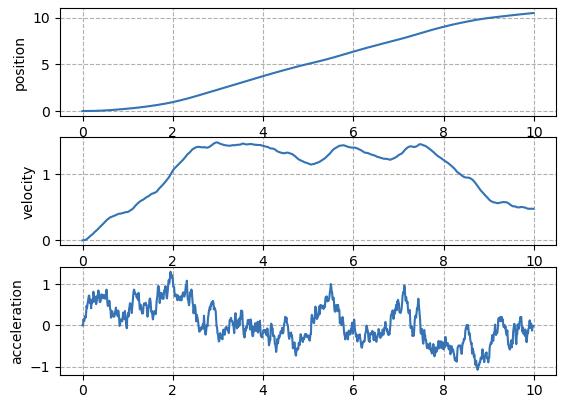
\includegraphics[width=0.56\textwidth]{images/ch1/01OU.jpeg}
    \caption{Change in displacement caused by a randomly generated OU process.}
    \label{fig:01OU}
\end{figure}   


\subsection{Stabilization of Training}
Architecturally, DDPG contains two interacting neural networks that are trained upon each other.  To successfully train such a complicated system, careful parameter initialization and proper weight updates are paramount.  Although some initialization techniques were introduces in the above sections, the authors of \cite{ddpg} initiated the last layer of the networks with weights uniformly drawn from $[-3 \times 10^{-3}, 3 \times 10^{-3}]$ for low dimensional problems. Such an initialization ensures initial policy and value estimates were near zero \cite{ddpg}. The other layers were initialized using uniform distributions $[-\frac{1}{\sqrt{n_j}}, \frac{1}{\sqrt{n_j}}]$, where $n_j$ was the size of the previous layer.  Regularization-wise, batch normalization was used \cite{batch_norm}. For exploration, the UO noise given in Equation \ref{eq:01OU} with $\theta$ and $\sigma$ as 0.15 and 0.2 was used.

\subsubsection{Experience replay}
DDPG also uses experience replay (sometimes called replay buffer) to enhance data efficiency and prevent catastrophic interference during training.  Experience replay was first introduced in \cite{exp_replay} to provide temporally de-correlated training samples to agents in time-series settings. In DDPG, tuples of:
$$(x_t, u_t, r_{t+1}, x_{t+1})$$
are memorized and stored in the experience replay. During updates, random mini-batches of previous experiences are sampled from the replay buffer to update the agent. Consequently, the agent obtains the ability to learn the same experiences many times, a concept similar to cycling through many epochs in deep learning. Correlating to humans, experience replay is similar to hippocampal replay, where memories are sub-consciously replayed over and over.  Indeed, that is one theory explaining the efficiency of human learning \cite{hippocampal}. However, human memories are rarely replayed randomly. Instead, only the most important or unexpected memories are replayed. Prioritized experience replay mimics this concept and biases sampling to experiences with large TD errors \cite{p_exp}. Intuitively, such experiences are \textit{shocking} since the outcome was significantly different than what was expected. Using prioritized experience replay, the agent learned faster in 41 out of 49 ATARI games compared to the original experience replay.

\subsection{Input and State Constraints}
As with all RL methods, input constraints can be handled quite trivially; however, state constraints are much more difficult. Typically, \textit{soft} state constraints are implemented in RL by introducing large negative rewards when the agent arrives at an undesired states. Indeed, humans learn state constraints in such a way where guardians provide negative consequences when we venture into troubling situations.  In literature, constrained Markov decision processes (CMDPs) and safe RL are two fields that explore how RL can handle constraints explicitly; however, most modern methods either require explicit system models or are difficult to implement in industry. 


\subsection{Training Algorithm}
The DDPG algorithm is trained as follows \cite{ddpg}:
\begin{enumerate}
    \item Initialize replay buffer and the actor and critic network weights corresponding to the previous subsection.
    \item Observe some states from the system 
    \item Map the states to some exploratory actions via the online actor network: $$\mu_t' = \mu (x_t | \theta ^{\mu}) + \mathcal{N}_t$$
    \item Implement $\mu_t$ to the system, observing transition to $x_{t+1}$ and obtaining $r_{t+1}$
    \item Store tuple $(x_t, \mu_t, r_{t+1}, x_{t+1})$ into the replay buffer
    \item Sample a mini-batch of $N$ experiences $(x_t, \mu_t, r_{t+1}, x_{t+1})$ from the replay buffer
    \item Using the target critic network, compute $y_t = r_t + \gamma Q'(x_{t+1}, \mu'(x_{t+1}|\theta^{\mu'})|\theta ^{Q'})$ for each experience
    \item Update online critic parameters by minimizing: $J = \frac{1}{N}\sum(y_i - Q(x_t, u_t|\theta^{\mu}))^2$
    \item Update online actor parameters by:
    $$\nabla_{\theta^{\mu}} J \approx \frac{1}{N}\sum \nabla_u Q(x, u|\theta^Q)|_{x = x_t, u = u_t}\nabla_{\theta^{\mu}}\mu (x | \theta^{\mu})|_{x_t}$$
    \item Update both actor and critic target networks:
    $$\theta^{Q'} \leftarrow \tau \theta^Q + (1 - \tau) \theta^{Q'}$$
    $$\theta^{\mu'} \leftarrow \tau \theta^{\mu} + (1 - \tau) \theta^{\mu'}$$
\end{enumerate}

Most steps above are intuitive to understand; however, steps 6 and 9 might be slightly confusing. In step 6, mini-batches of experiences are used for training to enhance data efficiency and to provide temporally de-correlated training data.  For time-series problems, such as continuous control, a direct adaptive control method like RL will quickly adapt to the current operating condition and exhibit catastrophic interference on other operating conditions.  By training on an uniformly sampled mini-batch of historical experiences, catastrophic interference can be largely avoided.

Step 9 shows the slow update of the actor and critic target networks.  This follows the same intuition as DQN, where the target network is frozen for periods of time to prevent the moving target problem.  Except in DDPG, the target networks are updated in small steps after each episode rather than being kept frozen, and then undergoing a complete update.



%%%%%%%%%%%%%%%%%%%%%%%%%%%%%%%%%% End Section DDPG %%%%%%%%%%%%%%%%%%%%%%%%%%%%%%%%%%%%%%%%
